% lambUserManualText.tex
% Main text of the user manual for the lamb ICU ventilator support software.
%!TEX root = UserManual.tex

\section{Introduction}
The \abb~ considers numerous scientific concepts for implementation within the network,
amongst which have been proposed studies of pediatric mechanical ventilation.  The management
of mechanical ventilators in the Pediatric Intensive Care Unit (PICU) is complex, both because of
the variety of modes of ventilation permitted by current vendors and because of the large
number of clinicians involved in the decision making.\\

[CONSIDER putting in stuff from Alan Morris' work, etc.  Kathy might want to write this, or Julie.  Idea
would be to give about a page of context.]\\

The software described in this User Manual has been developed in Java, using JBoss Drools as the inference
engine that creates advice for the clinician.  The software runs on laptop computers and stores the data locally, or
optionally may be connected to a central database server.  The rules that are used by the inference engine are designed
separately from the underlying Java code that provides the user interface.\\

There are two general modes of use for the software, administrative and bedside user.  The purpose of the administrative
mode is to allow the creation of user accounts, to enable setup of study preferences, and to manipulate the database
settings.  This mode also permits visualizing the rules that were fired for specific decisions.  The normal bedside user
mode prevents accidental destruction of the databases, and does not allow creation of new users.\\



\section{Installation}

The software is provided as a zip file that is decompressed with standard software.  Your computer must have a Java 1.6 
runtime installed or this software will not run.  Satisfactory performance has been obtained with vintage 2007 PC laptops.
Versions of the software are available for Windows, Linux, or OS X.\\

Start the application by double-clicking the icon, and a login screen will appear (Figure \vref{fig:splash}).  You will
also see (briefly) a window indicating that the knowledge engine is being created, which requires up to a minute. After this disappears, you will be presented with the login dialog, where you enter your name and password.  Click on the OK button to 
start the program.

\begin{figure}[htbp] 
   \centering
   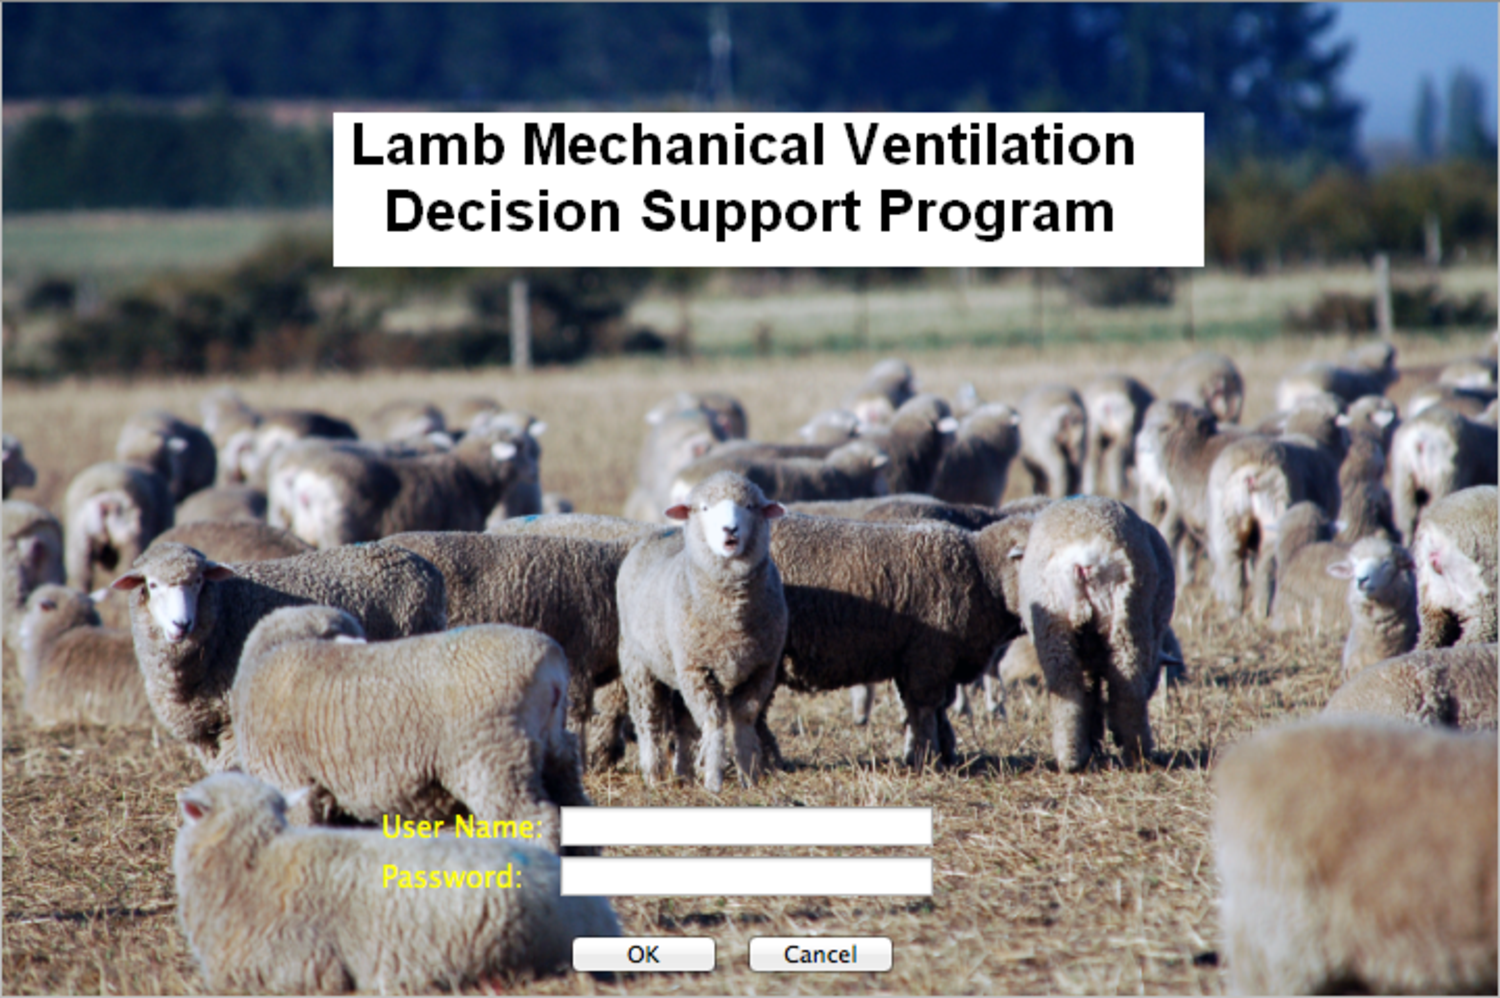
\includegraphics[width=\textwidth]{LoginScreen} 
   \caption{Login screen for decision support program.}
   \label{fig:splash}
\end{figure}

\section{General Navigation}

When you log in successfully, the software will display an interface similar to Figure \vref{fig:appBeforeMode}.  This figure
shows what an administrative user will see.  The normal bedside user view is very similar.  The only differences are absence of 
some of the menus, absence of the Property View, and absence of the Rule Trace tab.

\begin{figure}[htbp] 
   \centering
   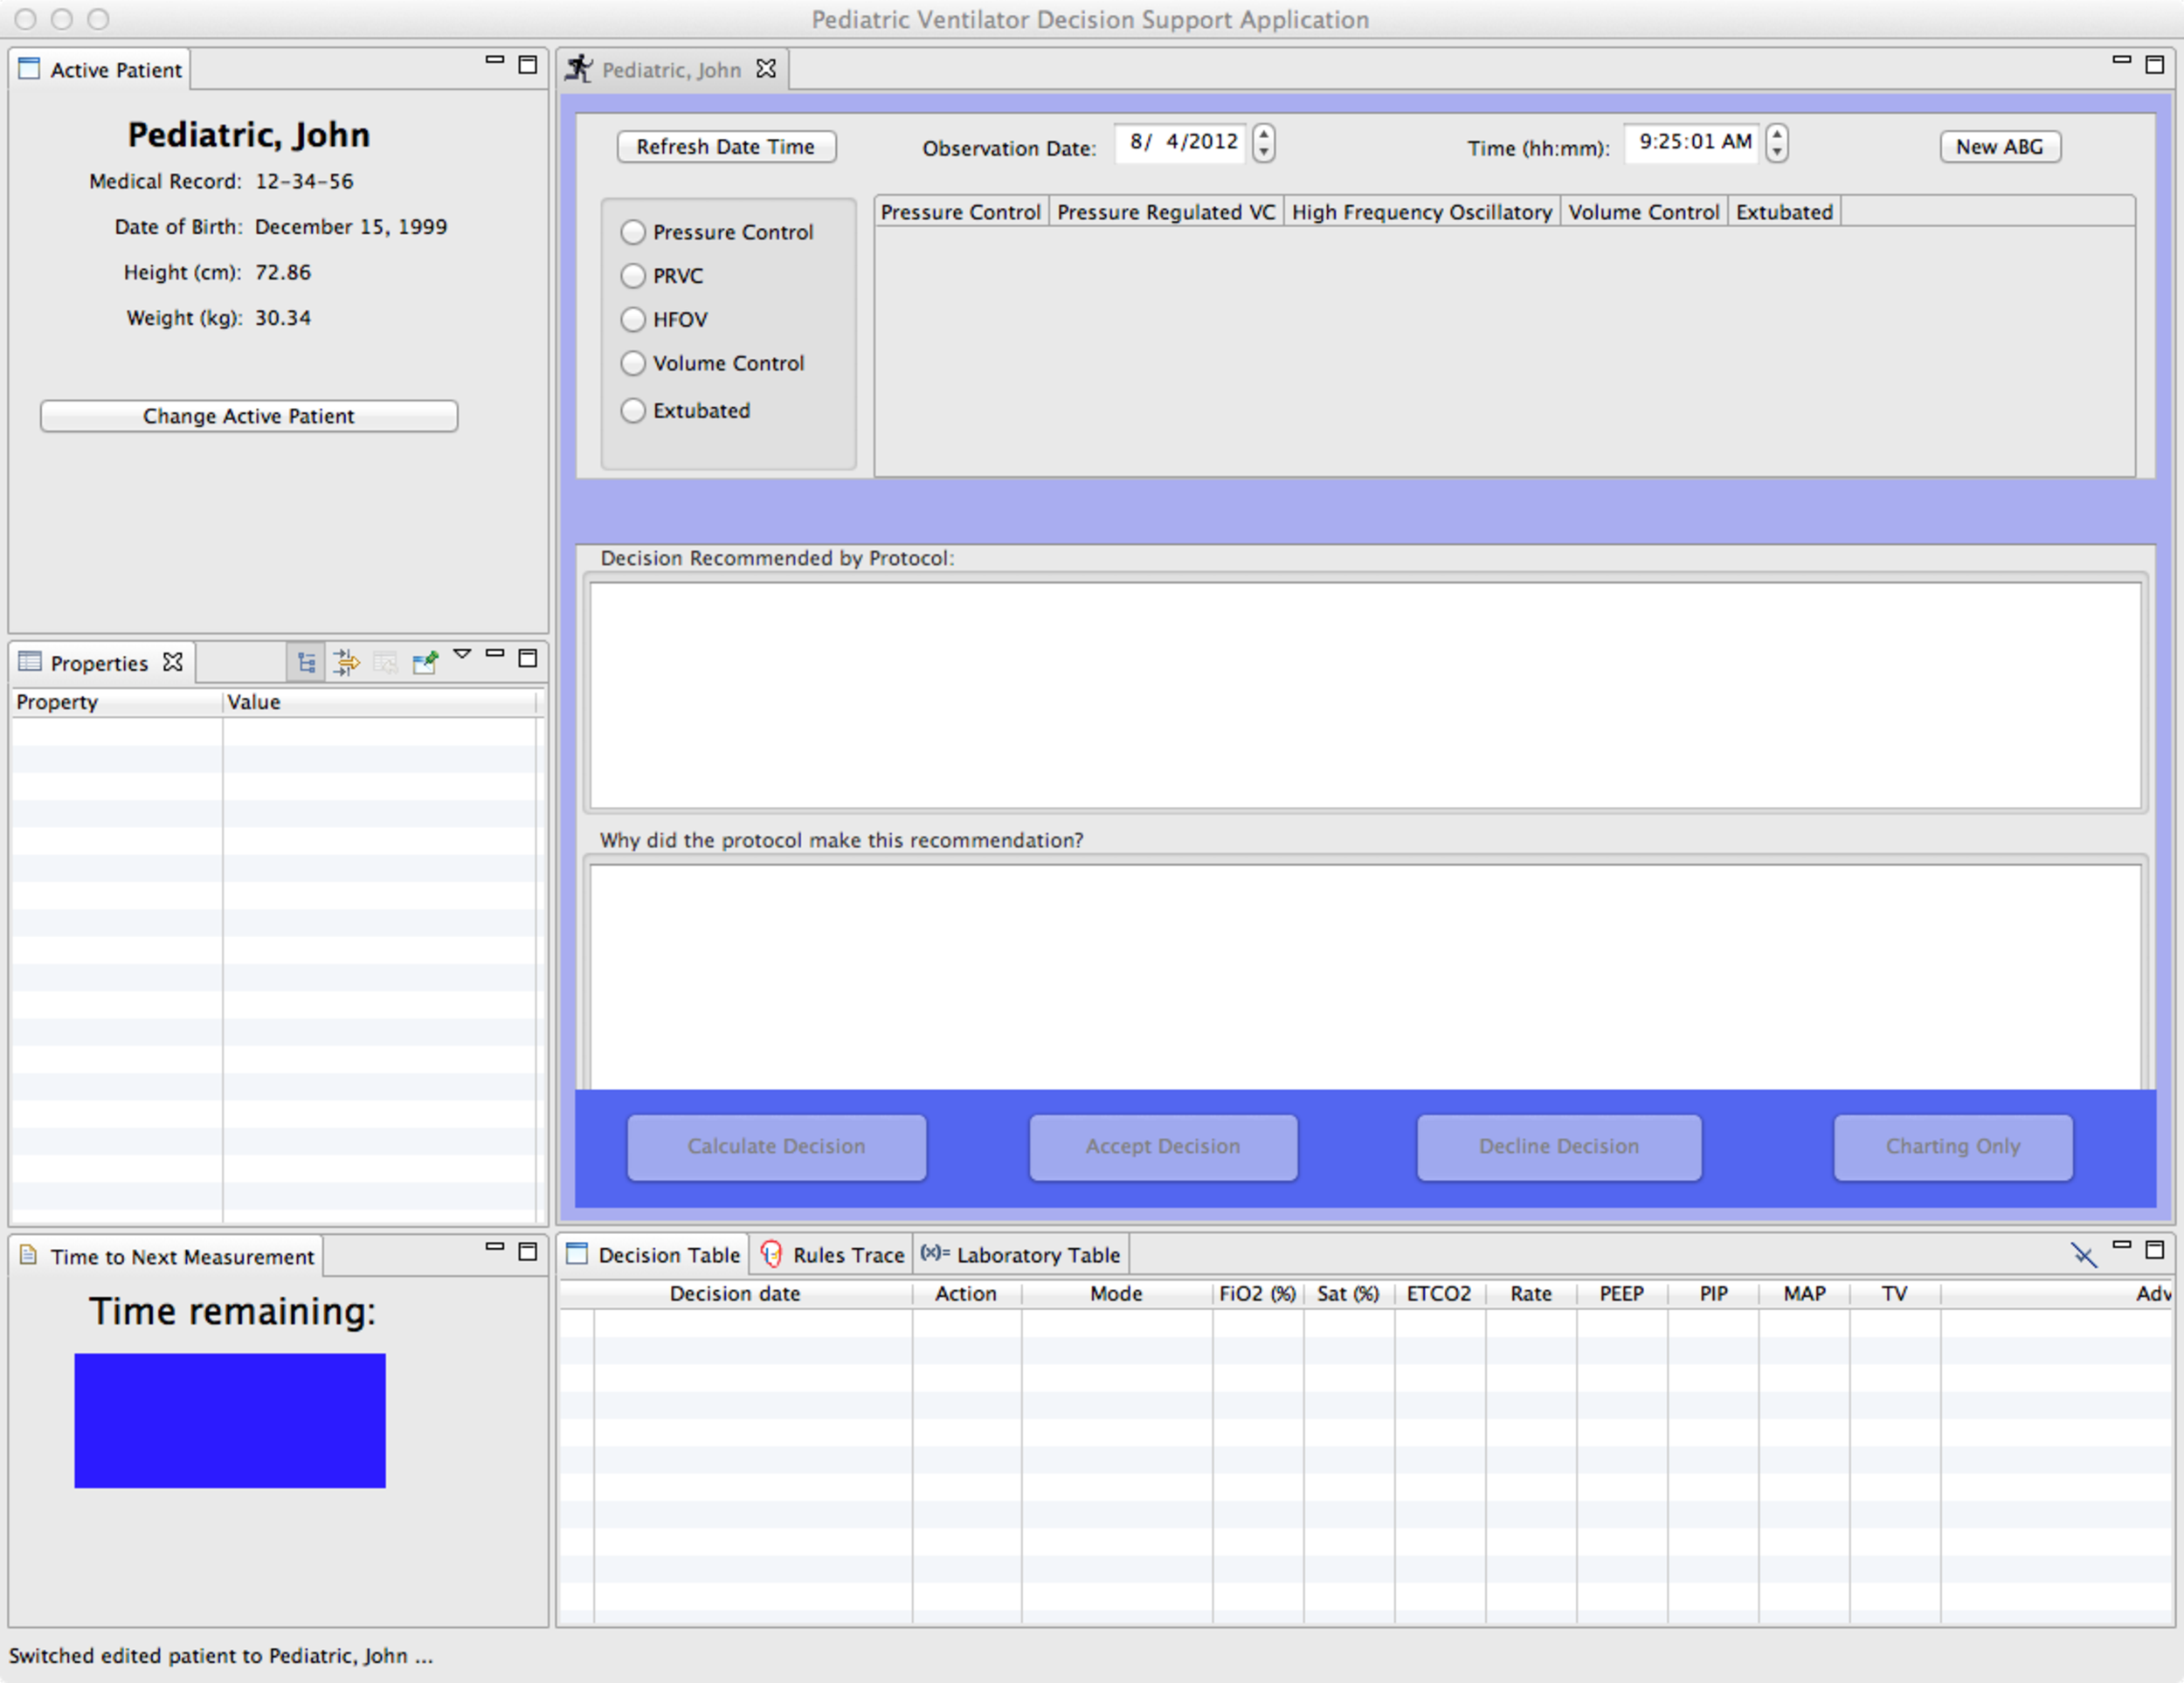
\includegraphics[width=\textwidth]{WholeAppBeforeModeSelect} 
   \caption{Graphic user interface of decision support software.}
   \label{fig:appBeforeMode}
\end{figure}

\section{Administrative Usage}

If you login as an administrative user, then you have the ability to create new users, set study preferences,
and manipulate the databases.  In addition, you are able to view the rule trace, which shows exactly how the
decision support was provided.

\subsection{Creating New Users}
To create a new user, click on the Database menu and select ``Add new user'' (see Figure \vref{fig:databaseMenu}).  


\begin{figure}[htbp] 
   \centering
   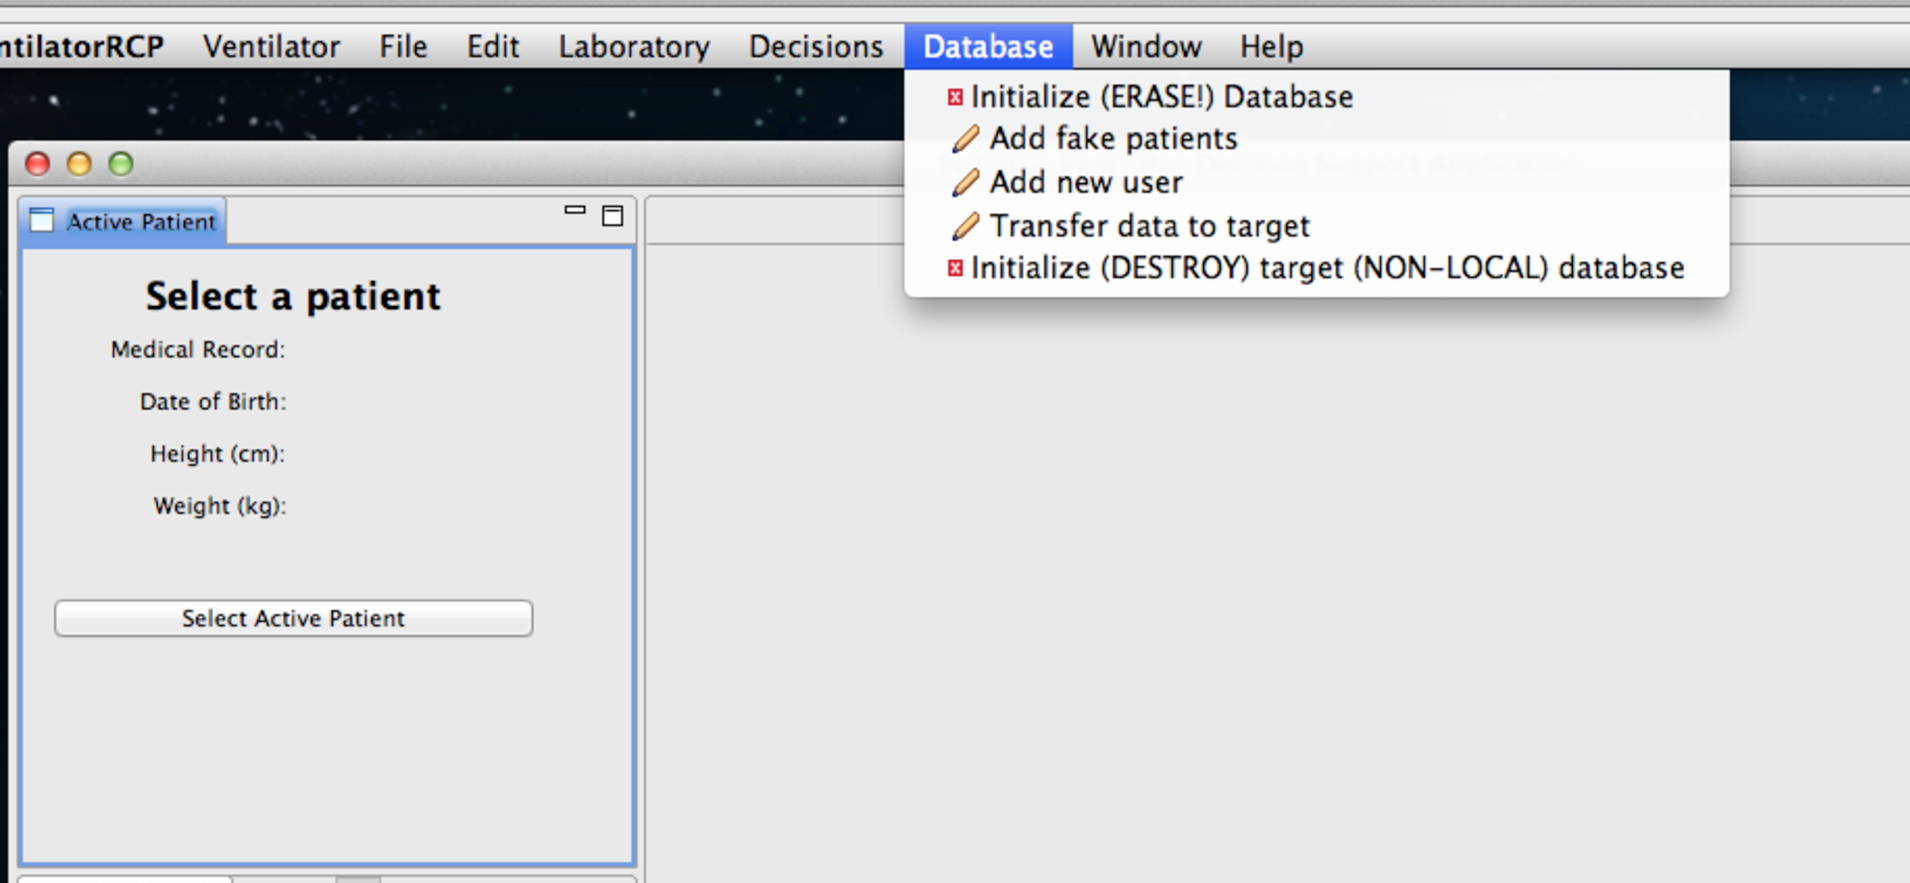
\includegraphics[width=\textwidth]{DatabaseMenu} 
   \caption{Database menu.}
   \label{fig:databaseMenu}
\end{figure}

 The computer
will display a dialog window in which you enter information about the user (Figure \vref{fig:newUser}).

\begin{figure}[ht] 
   \centering
   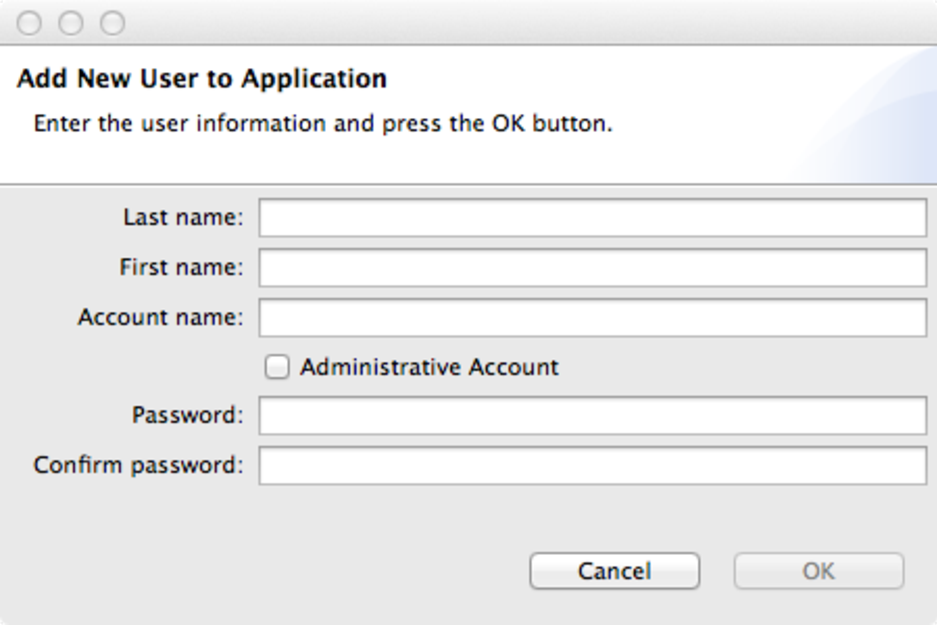
\includegraphics[width=\textwidth]{NewUserDialog} 
   \caption{Dialog window for entering new user information.}
   \label{fig:newUser}
\end{figure}

You should enter the last and first names of the new user, and then enter the account name
which will be used for logging into the software.  You will indicate whether the account is
an administrative account by checking the Administrative Account checkbox.  Enter the password
for the user.  Note that in the current version of the software, the password cannot be altered and
you will need to provide the password to the new user.



\subsection{Setting Preferences}
If you select the Preferences menu item (location differs by computer platform), you will see that there
are four categories of preferences.  Two of these are being used by the developers and you should ignore these (Drools Preferences
and Pediatric Ventilator Decision Preferences).  In the future, the Drools Preferences will control updating
decision rules from the Internet, and the Pediatric Ventilator Decision Preferences will allow selection of
International Units for international users.

\subsubsection{Database Preferences}

Select the Database Preferences  item from the Preference list.  The Database Preferences dialog will be displayed (Figure \vref{fig:dataPref}).  
The software has an embedded HSQLDB database for storing data locally on your computer.  Optionally, you may
choose to store data on a MySQL Server, in which case you should enter the connection settings for your
MySQL database.  Leave the Hibernate Dialect unchanged.  Be careful because the decision support software will not
create the MySQL database if it does not exist.  In MySQL, you must create an empty database with the name provided in
the settings.  The software WILL create the required table structure when you initialize the database (Section \vref{section:dataManagement}).\\

The target database is a database to which you can transfer data from the main working database.  For example, you may
store your patient data on the local HSQLDB database or the MySQL database that you set up in the previous step, but
wish to send all the data to a central research database (the target).  This would be the typical situation in
multi-institutional studies implemented by \abb~.  You would probably set up a MySQL server in your PICU to store all
the local data, and the target database would be at the Data Coordinating Center.  Encryption options are available to 
reduce transmission (to the target database) of patient identifiers (Section \vref{section:studyPreferences}).\\

\begin{figure}[htbp] 
   \centering
   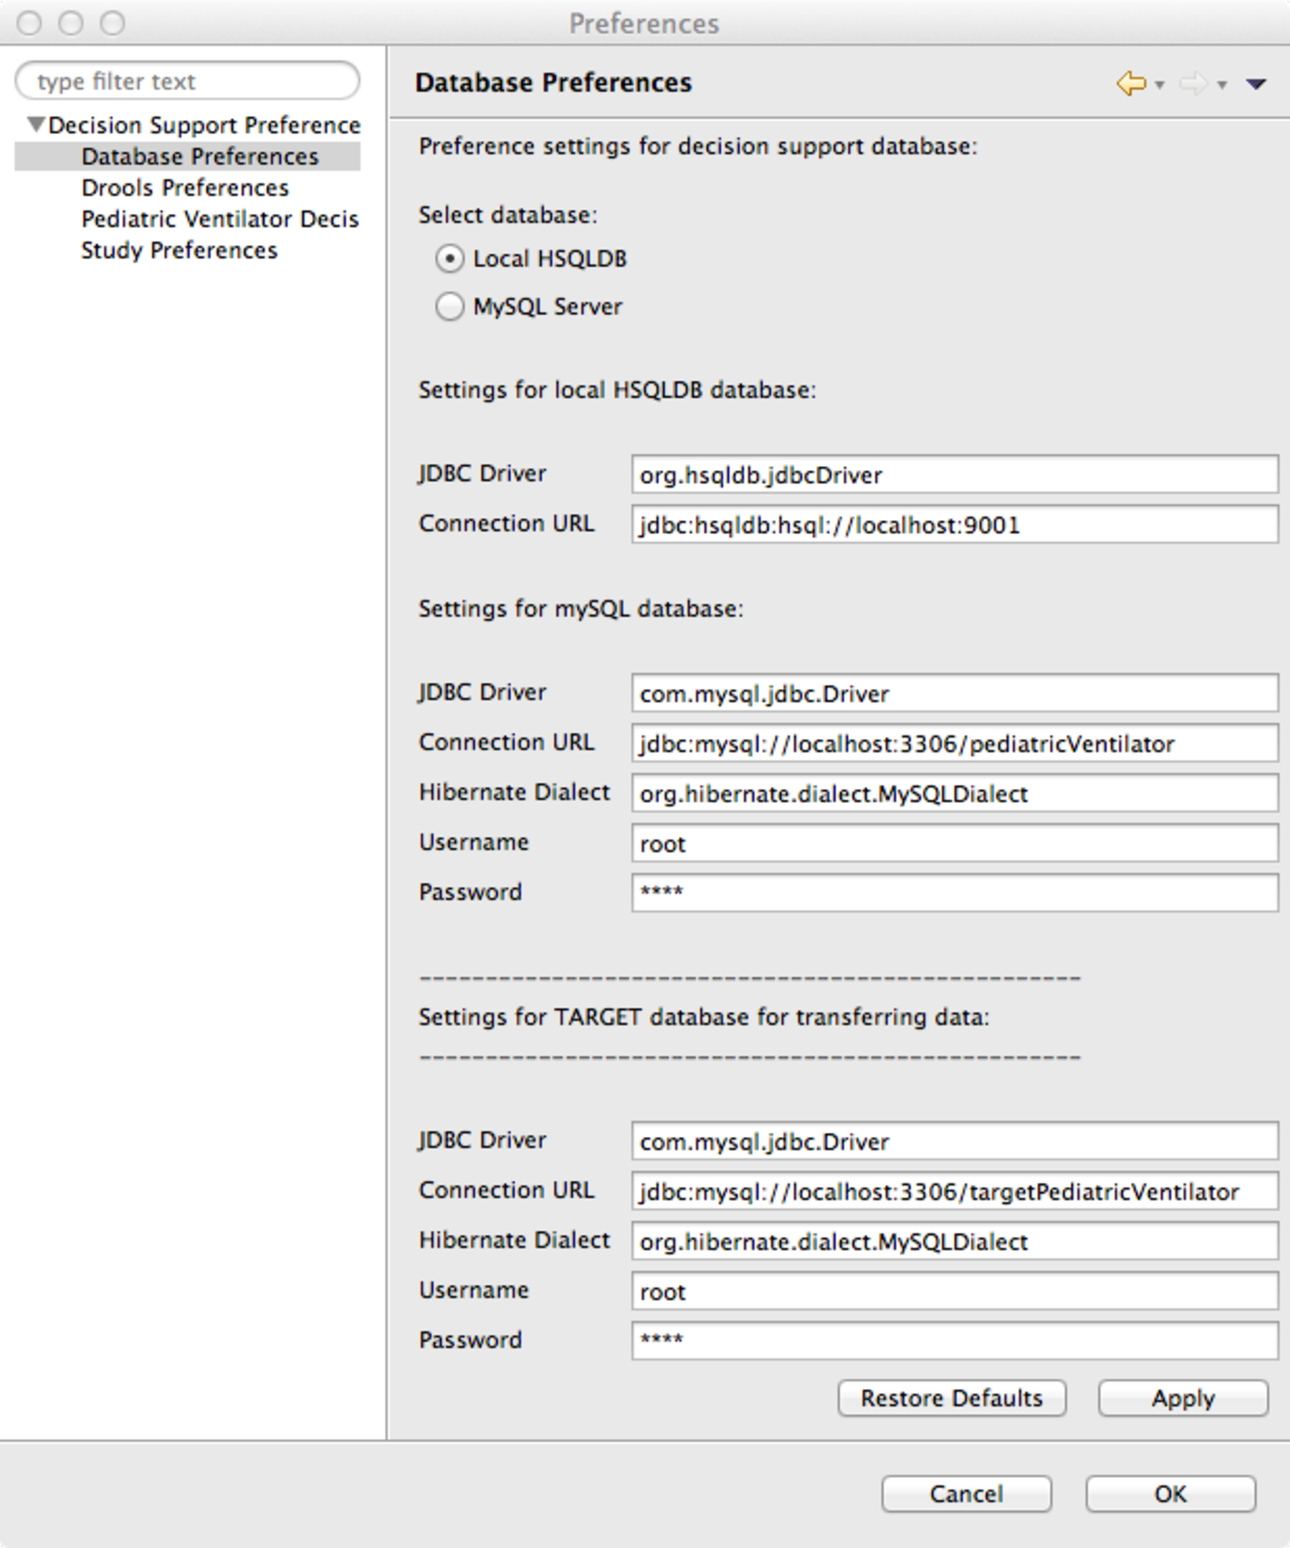
\includegraphics[width=\textwidth]{DatabasePreferences} 
   \caption{Database preferences dialog.}
   \label{fig:dataPref}
\end{figure}

If you are uncertain how to set the database preferences, you may leave them unchanged and the local HSQLDB 
database will be sufficient.  When you are ready to combine data from multiple patients, however, you will need
to set up the target database.\\

After you have finished editing the settings in the dialog, click the Apply button and the OK button.  If you wish
to restore default settings, you click the Restore Defaults button.  Of course, you may Cancel your choices by
clicking the Cancel button.

\subsubsection{Study Preferences\label{section:studyPreferences}}
Select the Study Preferences item from the Preference list.  The Study Preferences dialog will be displayed
(Figure \vref{fig:studyPref}).
The top section of the dialog determines how study subjects are numbered.  The default setting is the simplest and
probably the correct setting if you are sharing research data outside your institution.  The Prefix of the study
site and the Prefix of the study name are used inside the study number, which simplifies combining data from
multiple centers.\\

The software can be run in active or passive mode, determined by the Active Mode checkbox.  If this is not checked, then
the software is in passive mode.  In this mode, users can enter data, but the computer software will not provide any
advice.  It will ask the user to enter the decision made by the user.  This is an important part of the software, because 
this allows collection of ventilator management data that is being used when there is no computer decision support.\\

If you check the Active mode checkbox, then the computer program will provide advice when you select the Calculate Decision button,
described in Section \vref{section:normalDecisions}. \\ 


\begin{figure}[htbp] 
   \centering
   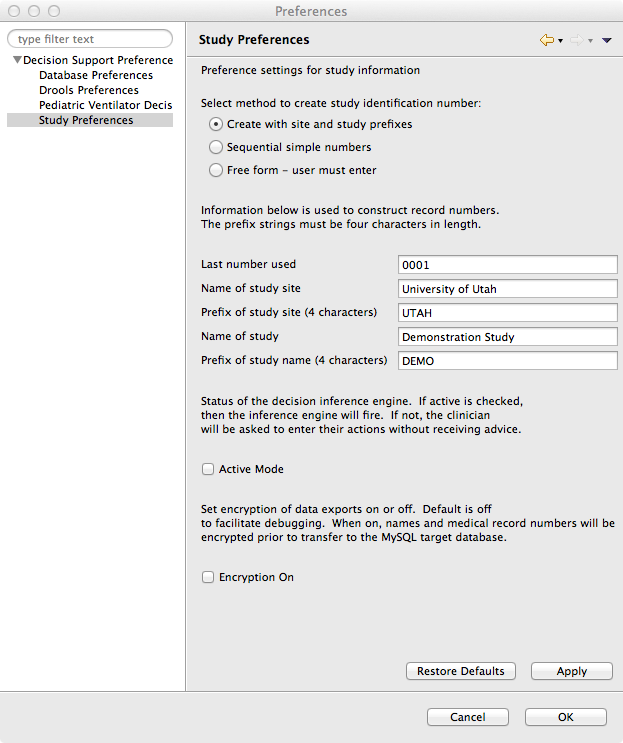
\includegraphics[width=\textwidth]{StudyPreferences} 
   \caption{Study preferences dialog.}
   \label{fig:studyPref}
\end{figure}

Finally, you can turn Encryption On by checking the Encryption On checkbox.  When this is checked, then names and medical
record numbers on the local database (or local MySQL server) are encrypted with a sophisticated one-way hash prior to
transmission to the target database (usually at the Data Coordinating Center).  While the same names and medical record numbers
will result in the same encryption, it is mathematically impossible to obtain the names or medical record numbers from the
encrypted information.  The hash is a one way process, so the privacy of your patients is fully protected when this setting
is selected.

\subsection{Database Management\label{section:dataManagement}}

The Database menu contains several actions in addition to Add new user, which you have already learned how to use.  The first one,
Initialize Database, will create a new database with the correct structure (tables) for the software to operate.  Notice, however, 
that initializing a database erases its contents (and starts over from scratch).  This is permanent (Figure \vref{fig:destroyData}).
The primary reason that this function is not available to normal bedside users is to prevent the accidental destruction
of study data with this command.\\

There is a Add fake patients menu item that is used by the developers to test the software.  If you are installing a version
of software on a demonstration machine, as you might do to teach people how to use the software, then you can add fake patients
with this command.  This can allow new users to learn how to the use the software without messing up real patient data.\\

The command to Transfer data to target will move the data on your local database to the target, which is usually
at the Data Coordinating Center.  This should be self explanatory.  It does \emph{not} erase the data from your local
machine.  If Encryption On has been selected in the Study Preferences, then the patients' names and medical record numbers are encrypted
before they are transferred to the target database.\\

Finally, the administrative user can erase the target database.  This is similar to Initialize Database in that it completely
erases the previous database.  This is a very dangerous command that will probably be removed from the software in later
versions.  If, for example, the target database at the Data Coordinating Center was connected to your machine, and you selected this
option, it would destroy the database at the Data Coordinating Center.  This option is present because there are no
current studies, and the software is still in development.

\begin{figure}[htbp] 
   \centering
   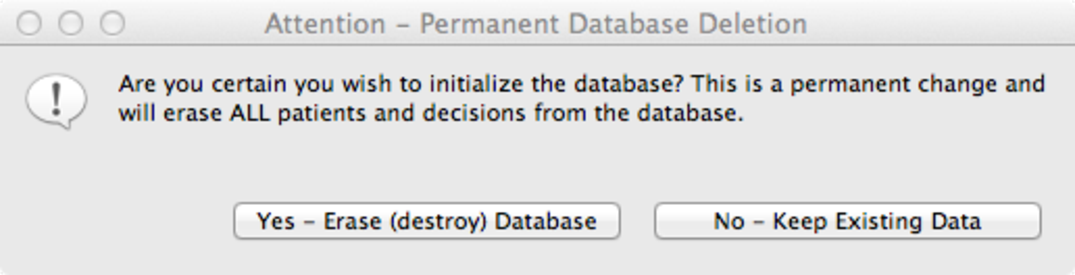
\includegraphics[width=\textwidth]{DatabaseDestroyAlert} 
   \caption{Study preferences dialog.}
   \label{fig:destroyData}
\end{figure}


\subsection{Viewing the Rule Trace}
The administrative user can also examine how the software reached its conclusions and constructed its advice
to the bedside user, by viewing the Rule Trace (Figure \vref{fig:ruleTrace}).  In future releases of this software, we
may move this function to the normal bedside user, because there is nothing dangerous about it.  The main reason
for it to be in the administrative mode is that this may be confusing to users at the bedside.

\begin{figure}[htbp] 
   \centering
   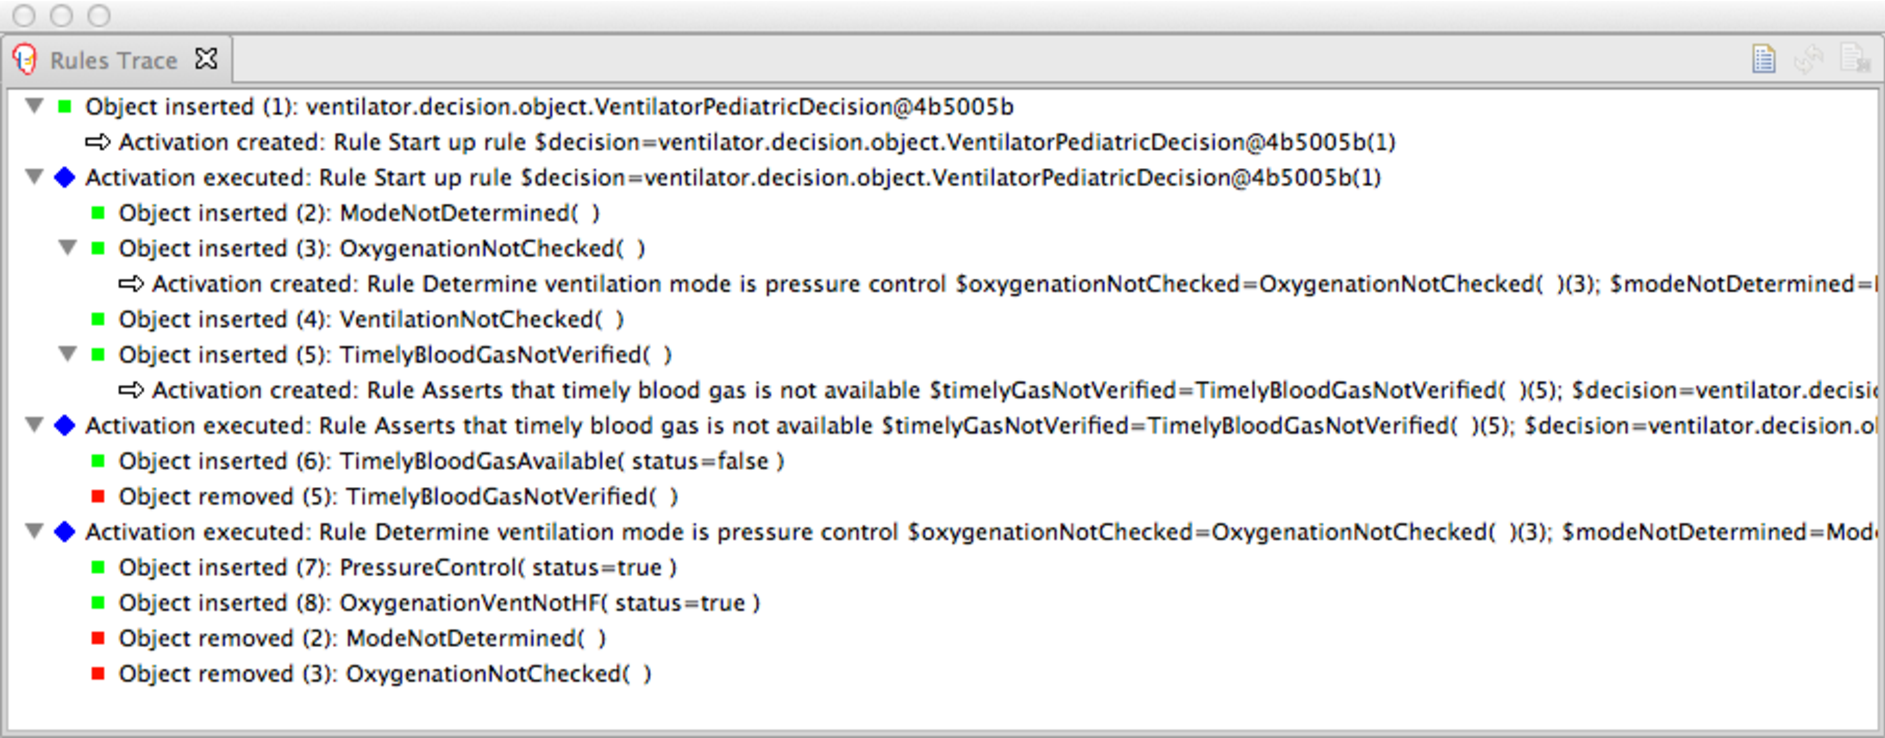
\includegraphics[width=\textwidth]{RuleTrace} 
   \caption{Rule trace view of decisions.}
   \label{fig:ruleTrace}
\end{figure}


\section{Normal Usage}

When you use the software as a normal bedside user, you need to be able to add or select a specific patient,
edit patient information, enter laboratory data, and enter information required for each ventilator decision.
After the software provides you with advice, then you need to accept or decline the advice.  You can also view 
the previous decisions and all the laboratory results that you have entered into the software.\\

\subsection{Creating, Editing, and Selecting Patients}
In the File menu, select New patient.  This will bring up a dialog for entering new patient information (Figure \vref{fig:newPatient}).  Notice that the date of birth is automatically initialized with the current date.  This
will be convenient in the neonatal setting or the Lamb Intensive Care Unit, but in normal PICU usage, you
will need to edit and enter the correct birthdate.\\

\begin{figure}[htbp] 
   \centering
   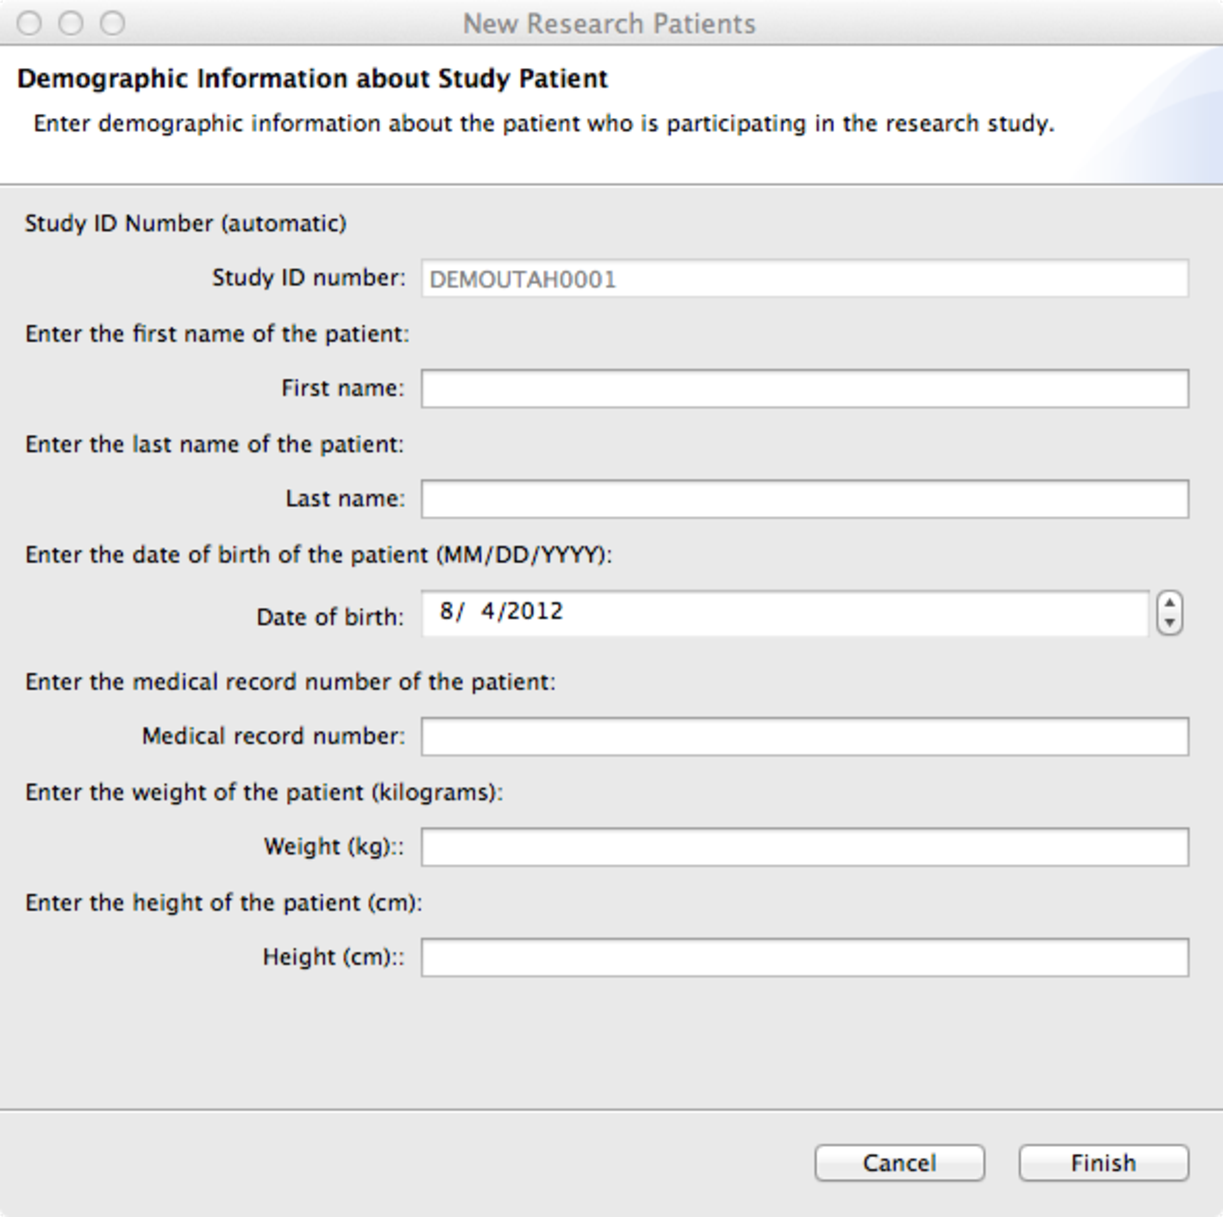
\includegraphics[width=\textwidth]{NewPatientDialog} 
   \caption{Entering a new patient into the software.}
   \label{fig:newPatient}
\end{figure}

When you start the software, there may be no patient selected, or perhaps the incorrect patient is selected.  You 
should click the button to Select (or Change) Active Patient.  This button is in the upper left section of
the software interface.  If there are patients in the database, a listing will be provided (Figure \vref{fig:patientList}).
Click on the correct patient, and click the OK button.  Alternatively, you may double click on the correct patient
and it will be selected automatically.

\begin{figure}[htbp] 
   \centering
   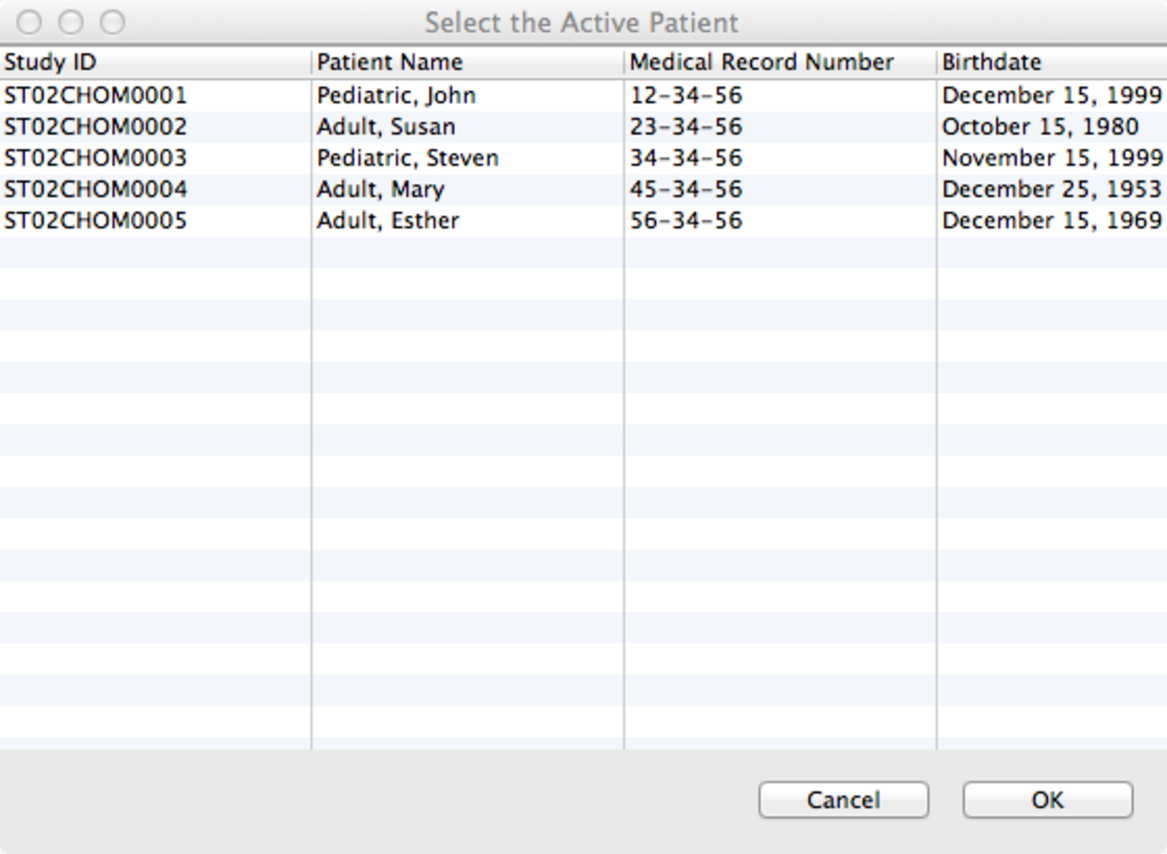
\includegraphics[width=\textwidth]{PatientListDialog} 
   \caption{List of patients in the database.}
   \label{fig:patientList}
\end{figure}

\subsection{Entering Laboratory Data}
To enter arterial blood gases, you may select the New ABG button on the upper left of the software screen, or you may use
the Laboratory menu and select Enter arterial blood gases.  Either method results in the Arterial Blood Gas Panel Result dialog 
(Figure \vref{fig:bloodGas}).  The date and time are populated with the current time, and you may need to edit these
variables.  The required measurements include inspired oxygen as well as the blood gas results.  \\

\begin{figure}[htbp] 
   \centering
   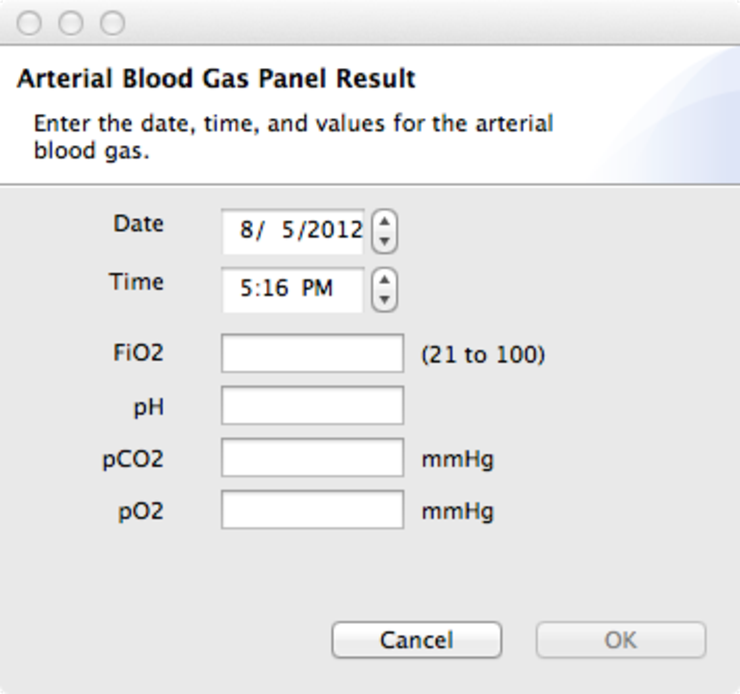
\includegraphics[width=\textwidth]{NewBloodGas} 
   \caption{Entering blood gas data.}
   \label{fig:bloodGas}
\end{figure}

After laboratory data have been entered, you can view them in the Laboratory Table in the lower section (center) of
the screen (Figure \vref{fig:labResults}).  The serum bicarbonate and base excess or deficit are calculated with standard equations.\\

\begin{figure}[htbp] 
   \centering
   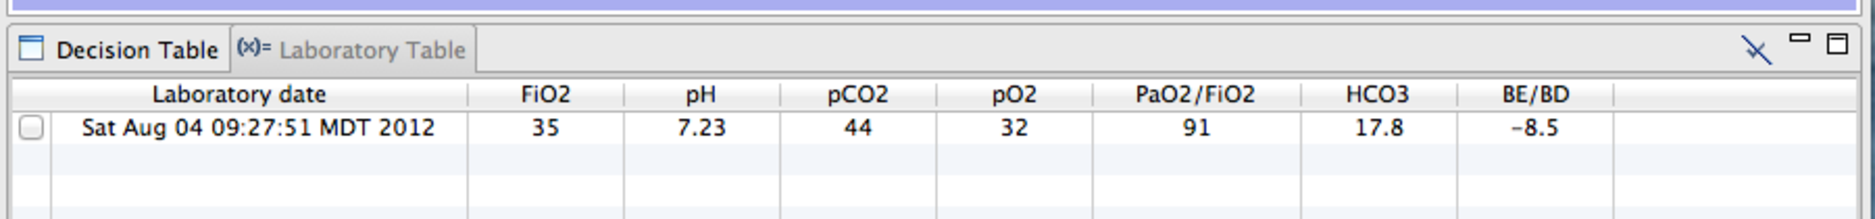
\includegraphics[width=\textwidth]{LaboratoryTable} 
   \caption{Laboratory table view.}
   \label{fig:labResults}
\end{figure}

\subsection{Obtaining Ventilator Decisions}
The purpose of the software is to handle ventilator decisions.  The first step is to select the mode of ventilation.  There
are five modes supported by this software:\\

\begin{compactitem}
\item
Pressure Control
\item
Pressure Regulated Volume Control PRVC)
\item
High Frequency Oscillatory Ventilation (HFOV)
\item
Volume Control
\item
Extubated
\end{compactitem}

The mode can be selected by clicking on one of the radio buttons, or by selecting
the appropriate tab.  In the Lamb ICU, you should select the Pressure Control mode.  Now the whole interface will be
filled in, similar to Figure \vref{fig:appPCMode}.\\


\begin{figure}[htbp] 
   \centering
   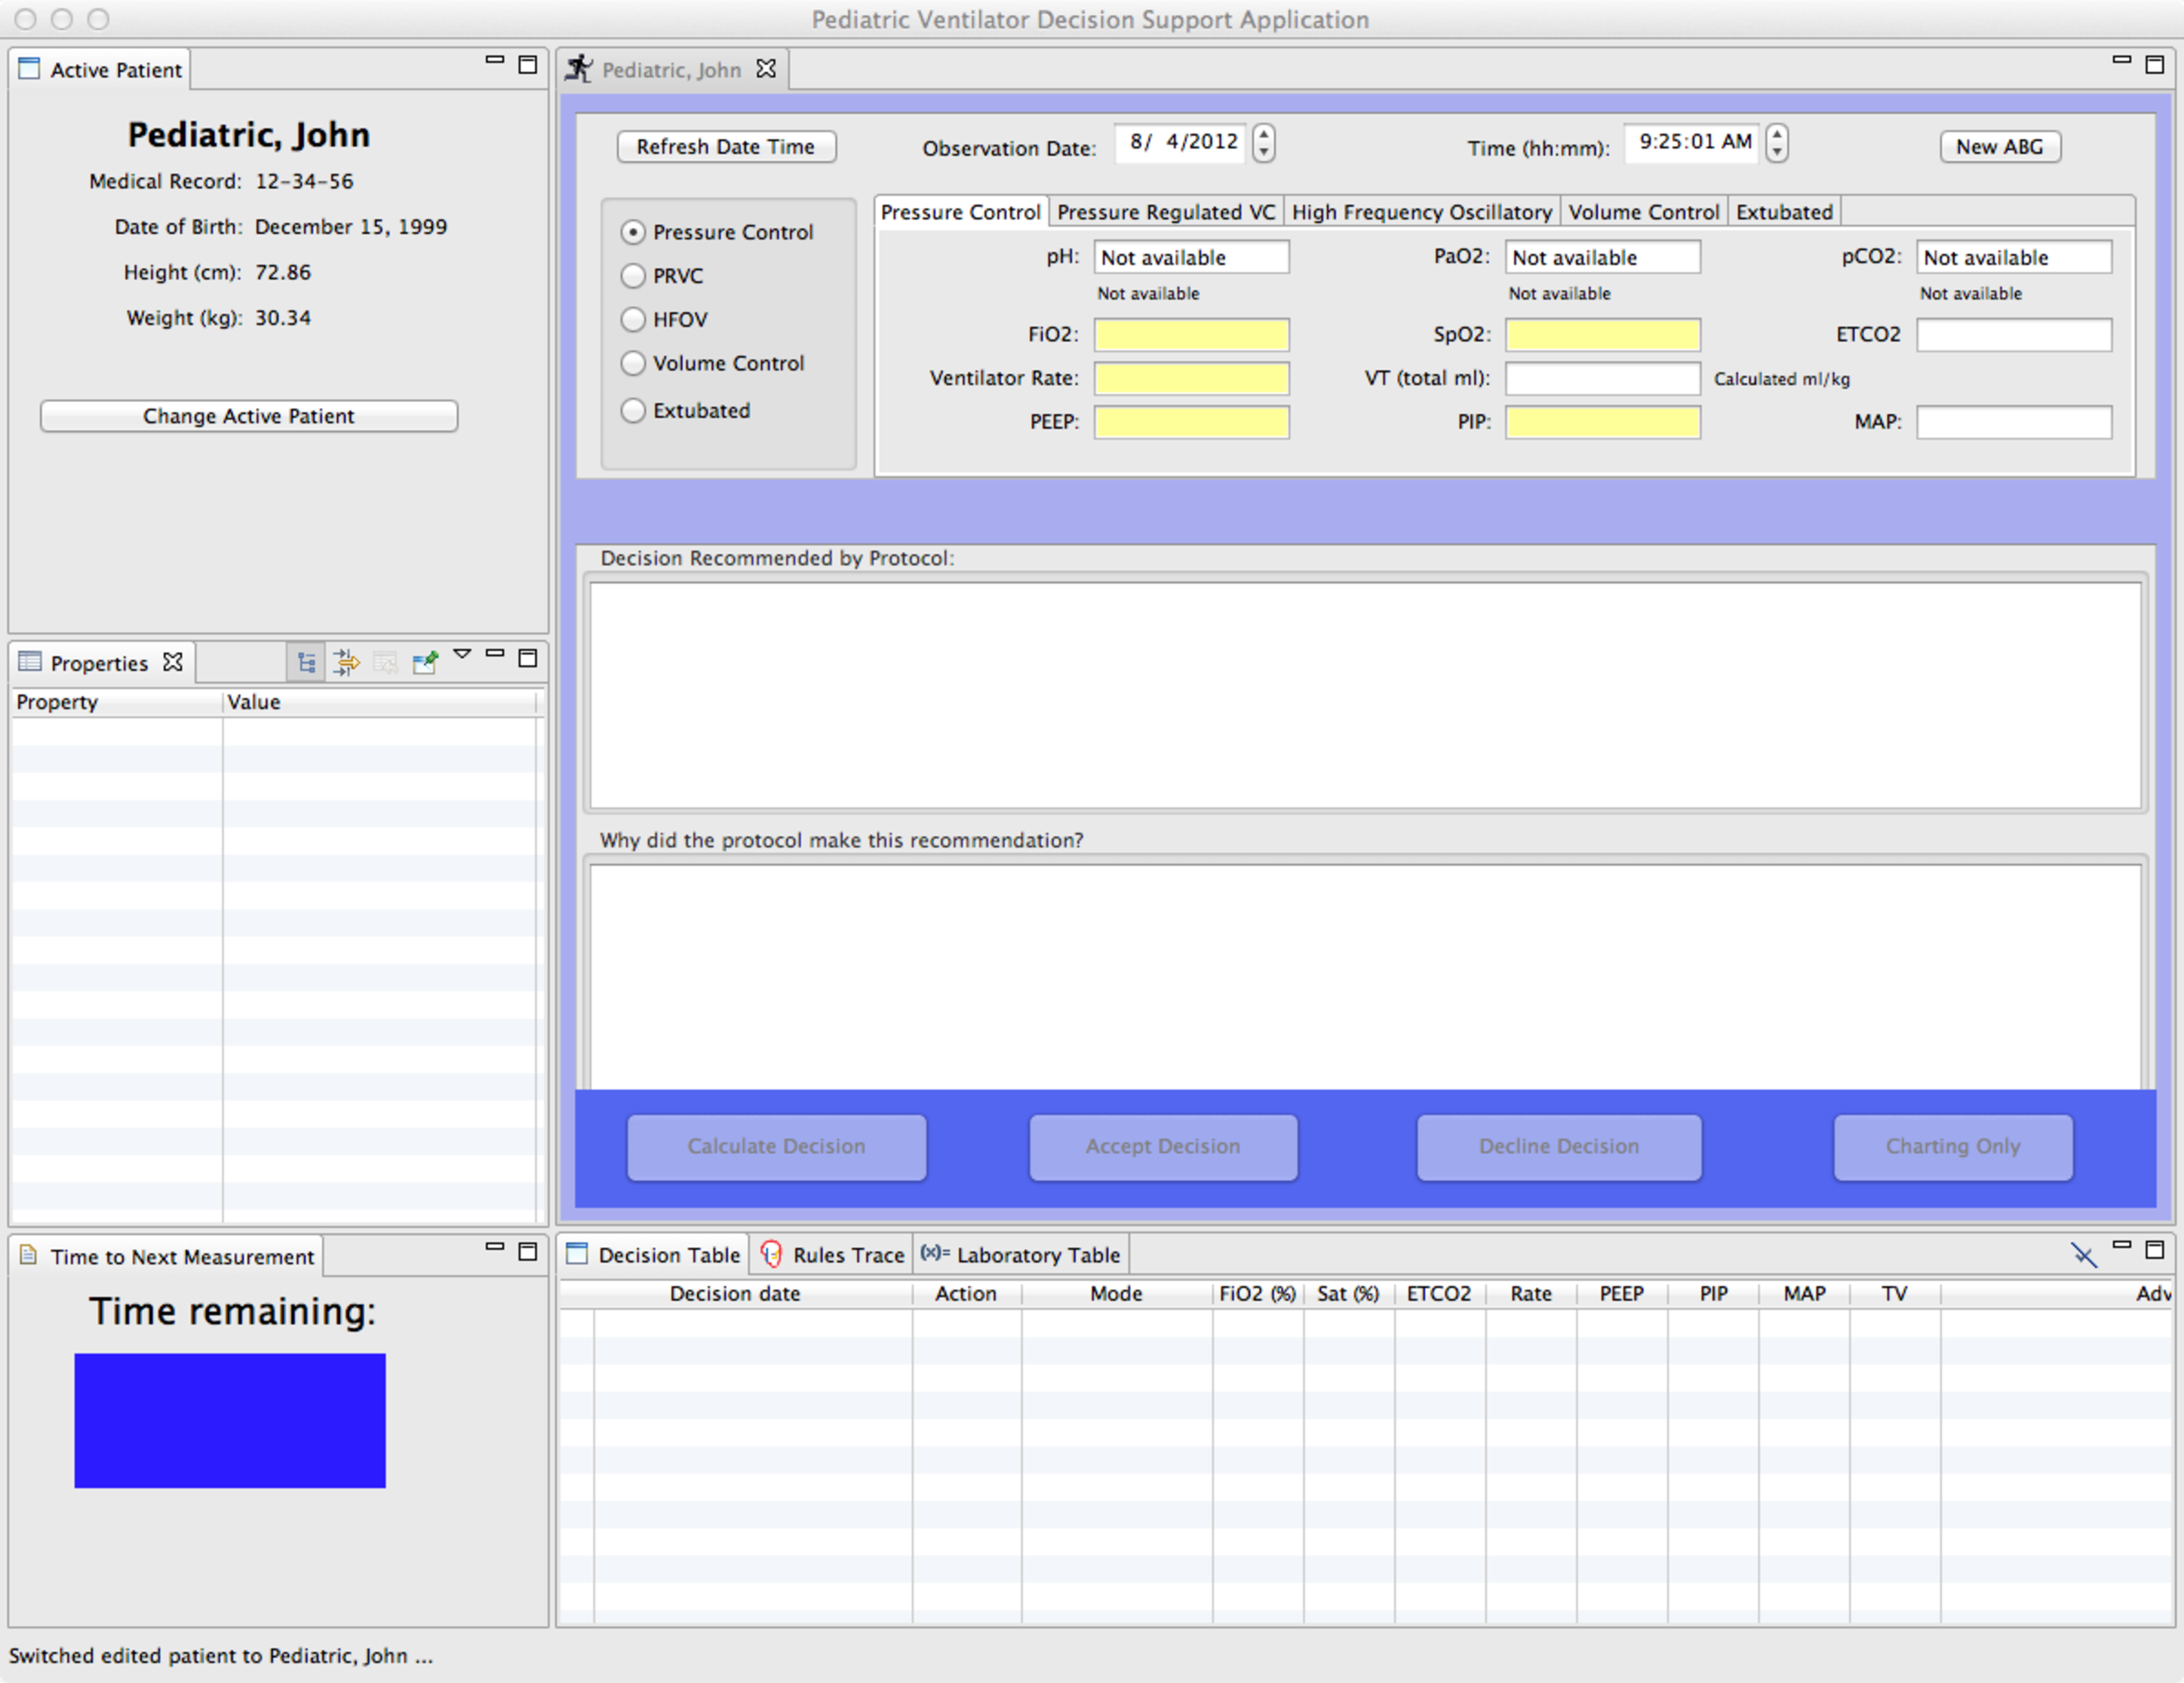
\includegraphics[width=\textwidth]{WholeAppPCMode} 
   \caption{Graphic user interface after pressure control mode selected.}
   \label{fig:appPCMode}
\end{figure}

Let's look at the variables for Pressure Control in more detail (Figure \vref{fig:PCZoom}).\\

\begin{figure}[htbp] 
   \centering
   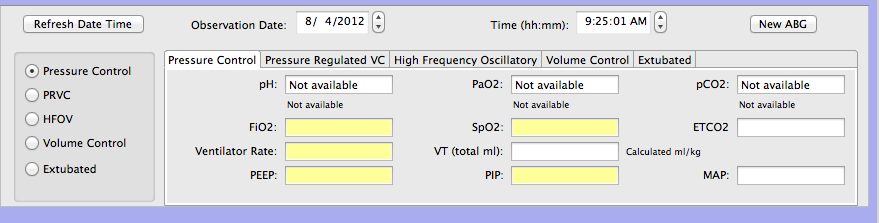
\includegraphics[width=\textwidth]{PC_Zoom} 
   \caption{Graphic user interface for pressure control ventilation.}
   \label{fig:PCZoom}
\end{figure}

At the top, there is a button for Refresh Date Time, as well as separate controls that you can use to edit the date
and time.  The Refresh Date Time button will set these controls to the current date and time.  On the upper right,
the New ABG will allow entry of a blood gas.\\

In the middle section, there is set of tab folders, one for each mode of ventilation.  The most recent blood
gas is displayed;  if there is no previous blood gas then these fields will be empty.  The subsequent fields
that are in yellow are required.  After you have entered the required fields, then the Calculate Decision button will
become enabled.  When that happens, then you can click on that button to obtain advice for your patient.\\

NOTE:  The current software will be changed so that SpO2 is optional (since it is not available in the Lamb ICU).  In 
addition, we know that we need to add an inspiratory time field.  This will be done before the software is officially
deployed in the LICU.\\

If the software is in passive mode, then when you click the Calculate Decision button, you will be asked to enter
the actual ventilator decision that you chose to make (Figure \vref{fig:actionTaken}). Filling this in accurately is
important because the software development team is using your current ventilator management to help
define rules to tell the computer how to develop advice for future users.\\

\begin{figure}[htbp] 
   \centering
   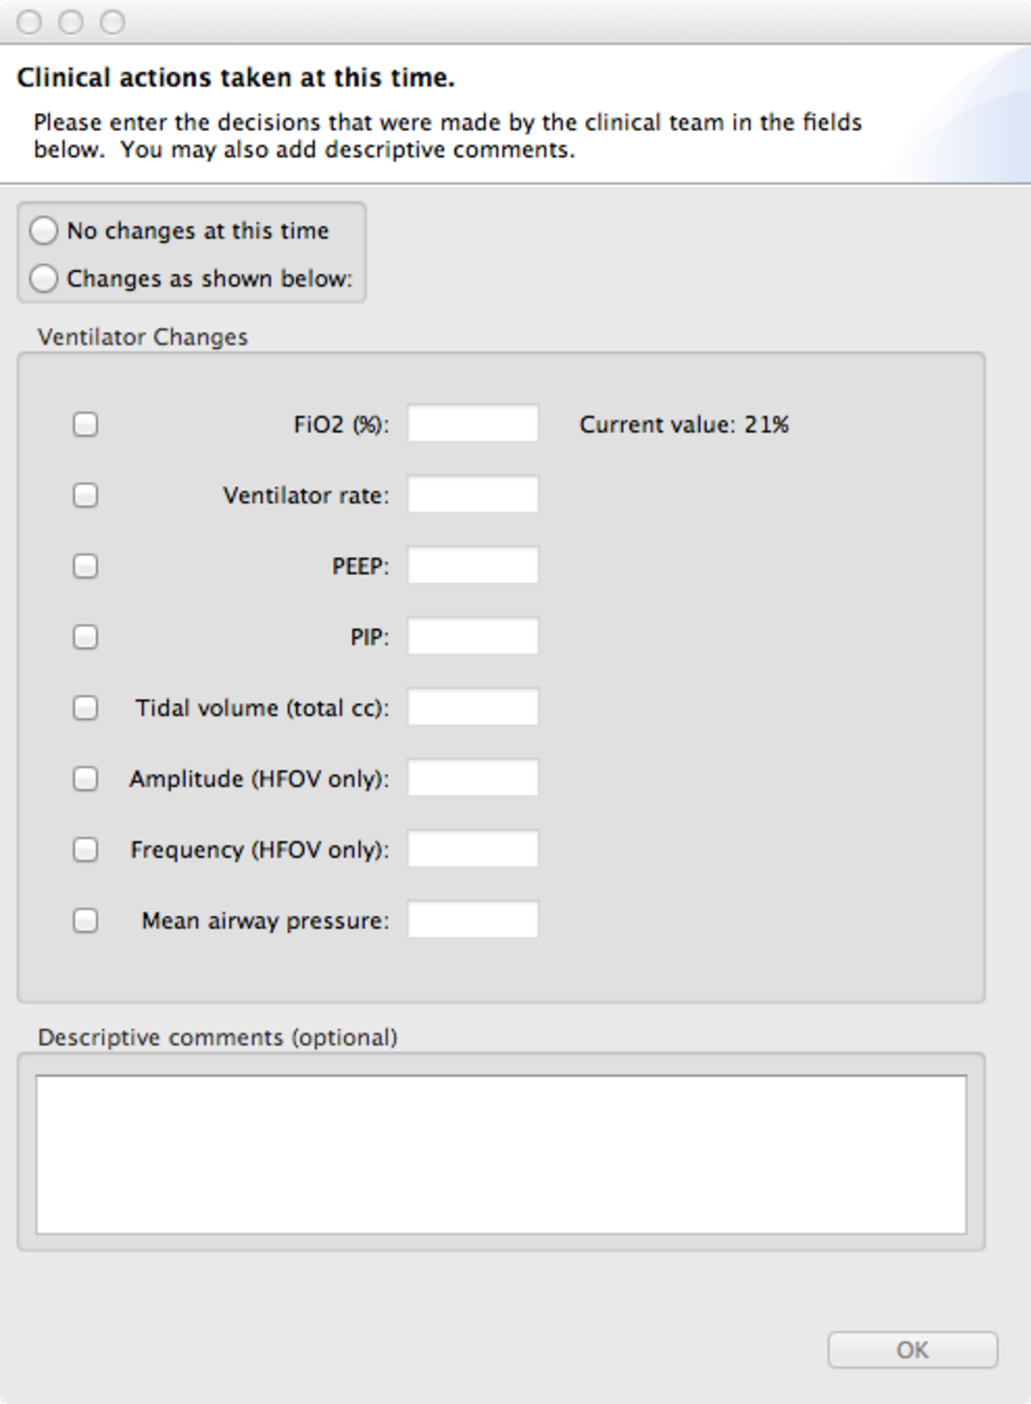
\includegraphics[width=\textwidth]{ActionTaken} 
   \caption{Entry screen for ventilator action taken.}
   \label{fig:actionTaken}
\end{figure}
 
If the software is in active mode, then when you click the Calculate Decision button, you will be presented with the
Decision Recommended by Protocol in the middle panel, and there should be an explanation in the panel below it.  At this
point, you can Accept Decision by clicking the appropriate button, in which case the decision is stored.  At this point,
the clock in the lower left of the screen will be reset and will count down to the time that you should enter the next
ventilator decision (or status).  \\

If you do not agree with all of the advice, you should click the Decline Decision button, and then you will be presented with
a dialog to ask you what you did, and why you disagree with the computer (Figure \vref{fig:decline}).  It is important
for you to realize that you are almost certainly correct if you do not agree with the computer.  The information you enter
at this point is critical for the developers to improve the software so that it makes better decisions.

\begin{figure}[htbp] 
   \centering
   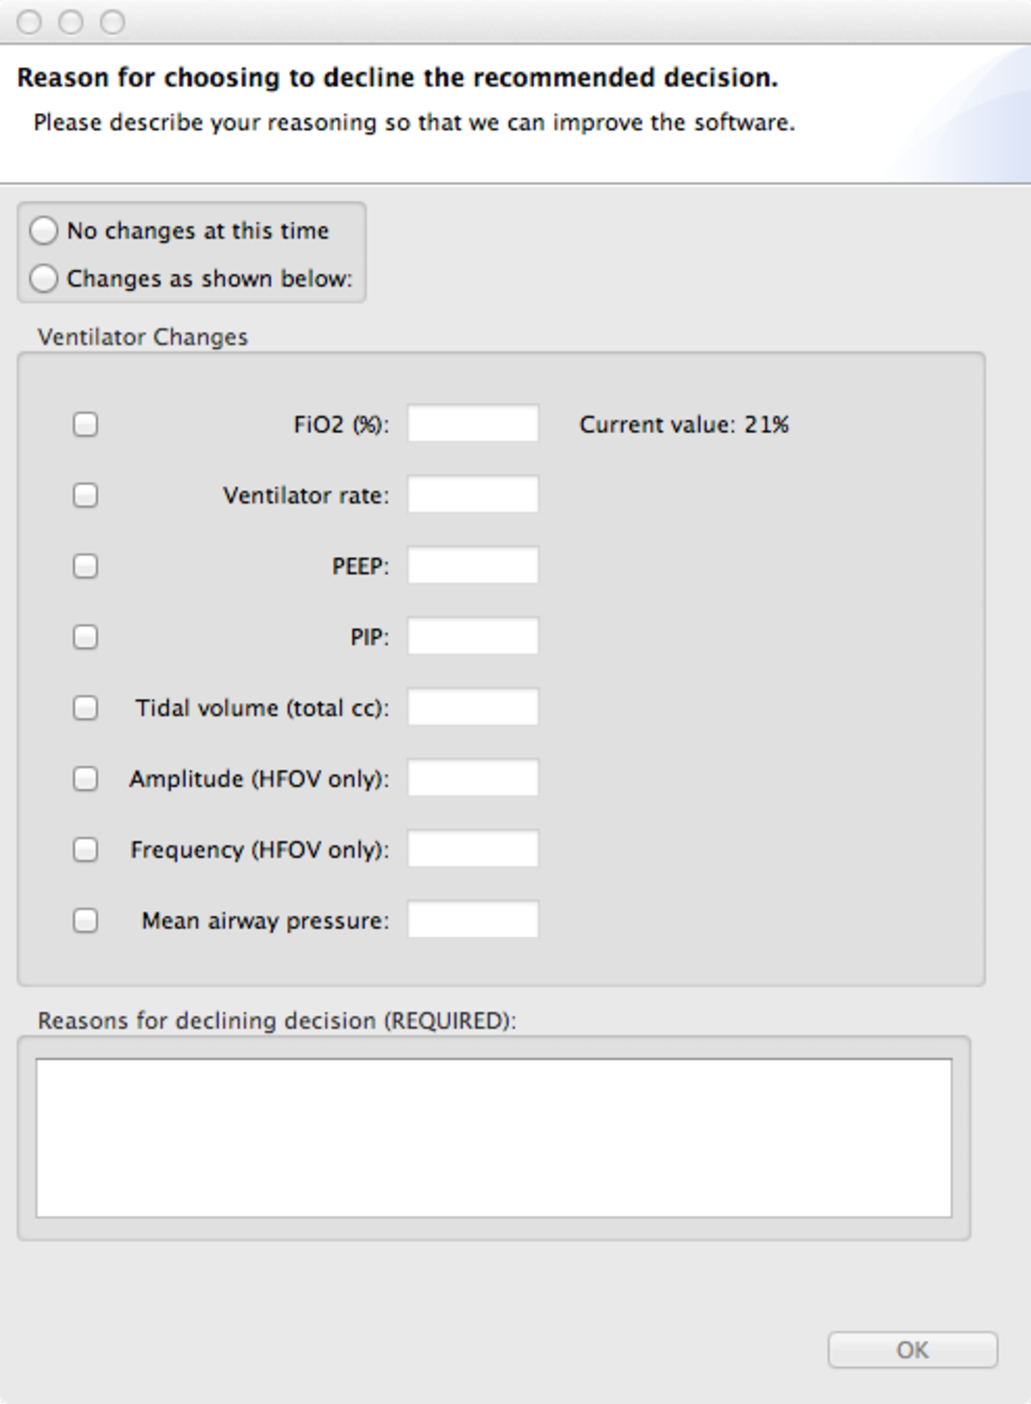
\includegraphics[width=\textwidth]{DeclineDecision} 
   \caption{Entry screen when user declines computer recommendation.}
   \label{fig:decline}
\end{figure}
 
\section{Summary}
This computer decision support software is a computer program in evolution.  You should not hesitate
to contact the authors with suggestions or questions.  Our immediate goals are to deploy working software in
the Lamb ICU at the University of Utah so that we can perfect the usability of the software, as well as develop
rules that will enable the software to provide reasonable recommendations for ventilator management.  In the future,
this software will be used in human subjects in the Pediatric ICU setting.  Your help now will enable this software
to reduce morbidity and mortality from ventilatory failure in children.

\endinput